\section{Climate model simulations}
\label{climate}

The Fourth Generation Coupled Global Climate Model (called CanCM4, here) produces a wide array of atmospheric conditions across the globe. Three experimental settings that are of particular interest are decadal, historical, and pre-industrial control runs. (Description of the type of simulations).

Decadal and historical simulations are run at $R=10$ different input settings. To obtain $R=10$ ``replicates'' for the control simulations, we randomly select ten non-overlapping 10-year periods. Our assumption is that each replicate is independent and has related extremal indexes within their respective simulation class.

We will look at daily winter precipitation and summer maximum temperature, both over California during the 1990s. The quantities used in the analysis are total precipitation (a weighted sum) and average maximum temperature (weighted). (Expand). This leads to a $R$ univariate time series for each class of simulations. To each time-series is fit a dynamic linear model (DLM) having the first two harmonics. Anomalies are computed by taking the difference of the time-series and the smoothed predictions based on the DLM. For winter we look at only December, January, and February. For summer we have June, July, and August. Finally, we treat the time-series as though there is no gap between the seasons of interest. For example, 28 February is followed immediately by 1 December in the winter analysis. This completes our pre-processing. (After the processing, the sequences are assumed stationary).

A comparison of each simulation class and likelihood is found in Figures \ref{figwinter} and \ref{figsummer}. (Not $K=5$ yet). In every situation we see that the estimates for $\theta$ are increasing with threshold (Check: Is this happening in the simulation study?). For a given likelihood, the means for the extremal index in each simulation class are roughly the same. We do not observe this for a given class: there is clearly a discrepancy between the estimates provided by the two likelihoods. However, in all cases, the 95\% probability intervals more or less overlap.

\begin{figure}
\begin{center}
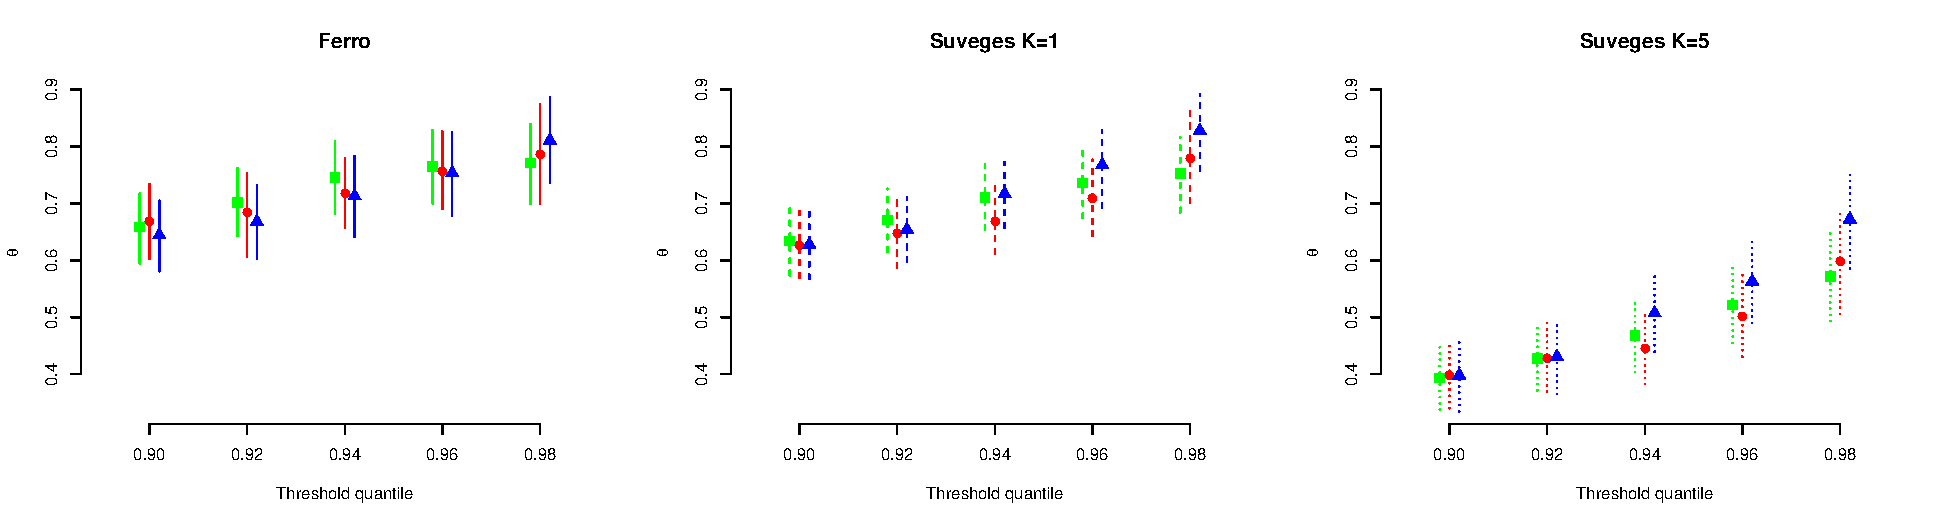
\includegraphics[scale=0.46]{figs/winter_like.pdf}
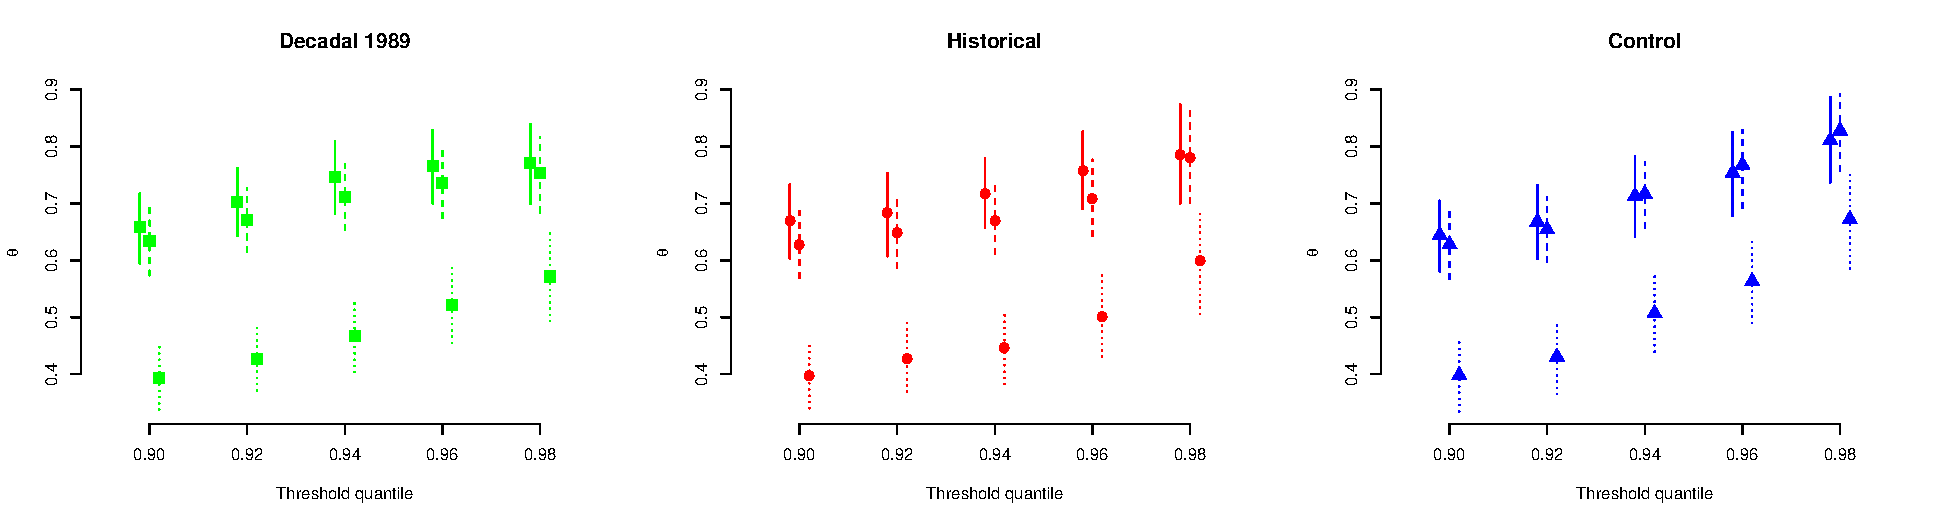
\includegraphics[scale=0.46]{figs/winter_source.pdf}
\end{center}
\caption{Both rows show the same information, but are arranged differently. The top row compares the extremal indexes of the climate models for a given likelihood. The bottom row compares the two likelihoods for each climate model. Solid lines (-----) denote model M1, dashed lines (- - -) denote M2 and dotted lines ($\cdot\cdot\cdot$) denote M3. Squares (\symsquare) mark decadal runs, dots (\symcircle) mark historical runs, and triangles (\symtriangle) are control runs. The points are the posterior means and the lines are 95\% h.p.d. intervals. The domain is California winter precipitation from 1990--1999.}
\label{figwinter}
\end{figure}

\begin{figure}
\begin{center}
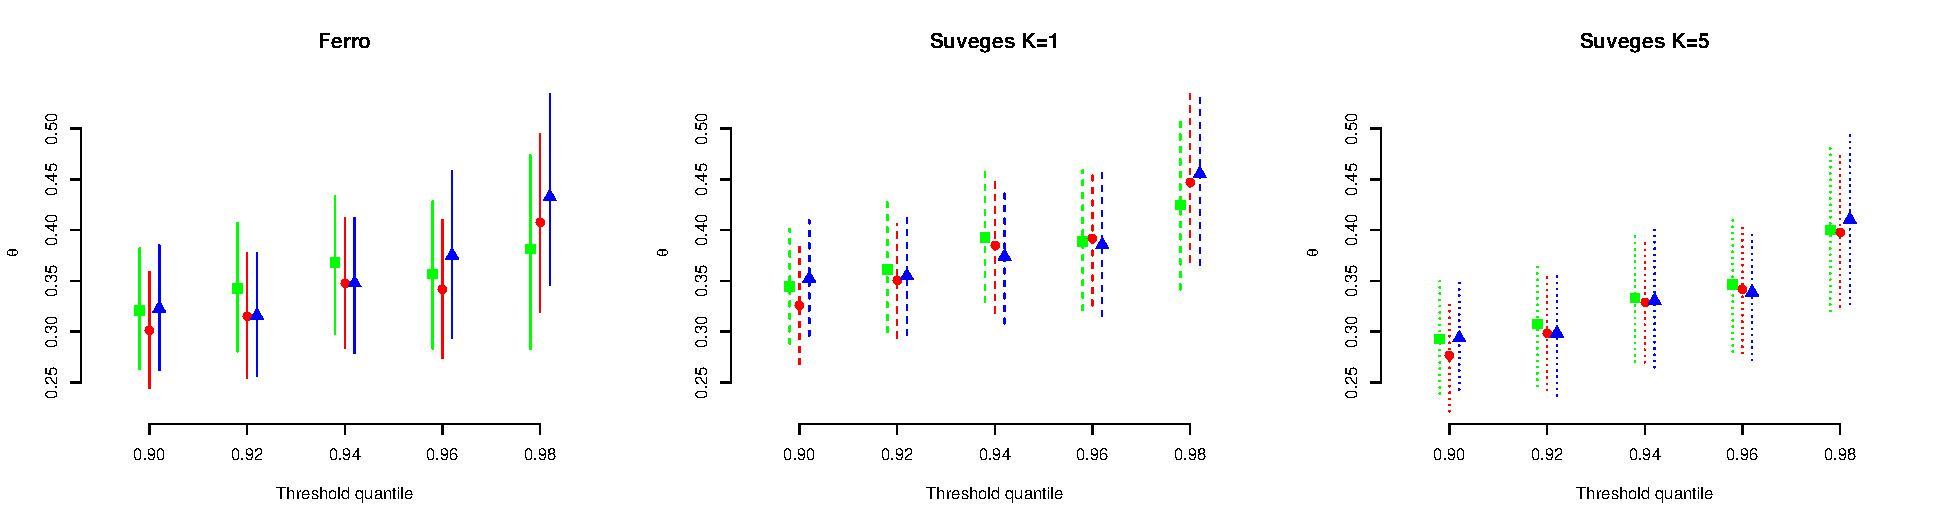
\includegraphics[scale=0.46]{figs/summer_like.pdf}
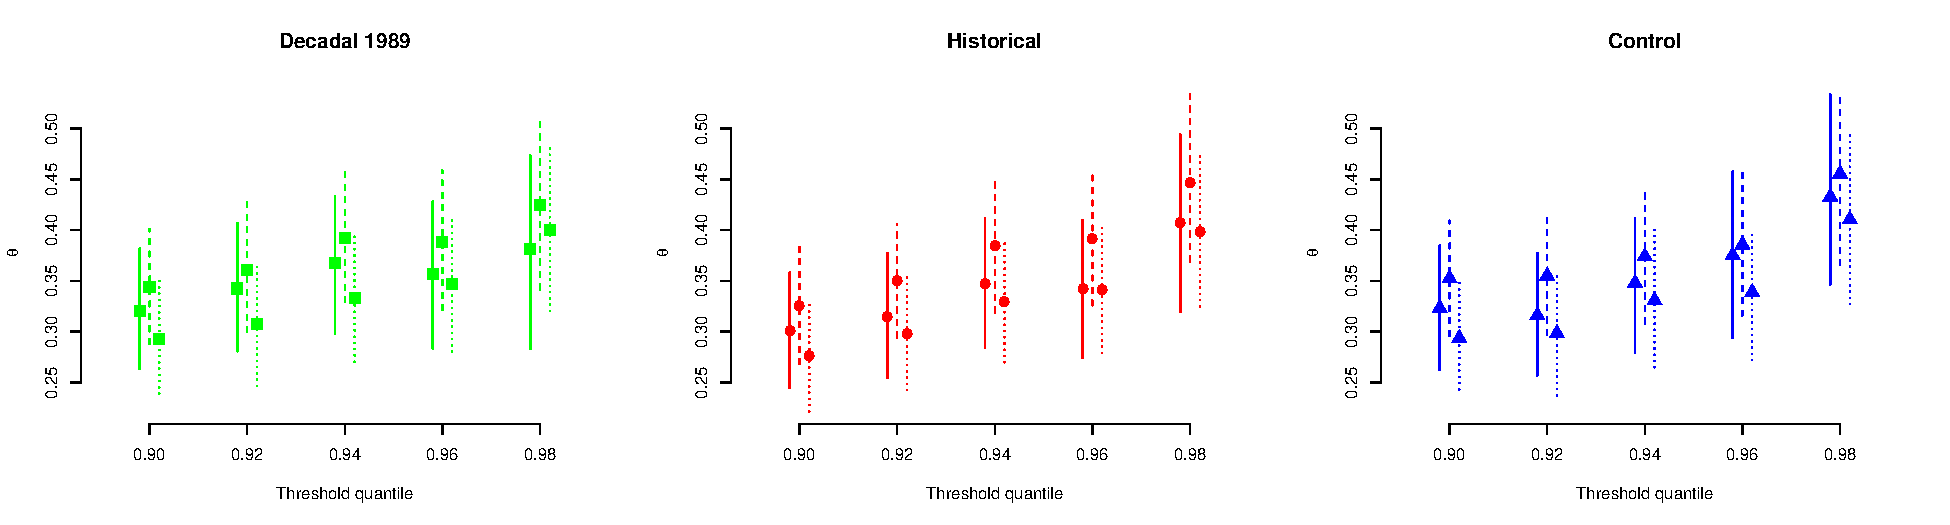
\includegraphics[scale=0.46]{figs/summer_source.pdf}
\end{center}
\caption{Same as in Figure \ref{figwinter}, but the hierarchical model is applied to summer maximum temperature.}
\label{figsummer}
\end{figure}

Where there is no overlap in intervals (see control runs for winter precipitation), we should consider how much of an issue this may be. Since the extremal index can be described as the reciprocal mean cluster size in the limit, there is a small practical difference between $0.63^{-1}=1.58$ and $0.83^{-1}=1.20$ when choosing to decluster the exceedances. The difference may be more pronounced when return levels are calculated. As $\theta$ decreases, non-overlapping posterior intervals become be much more concerning.
